\documentclass[]{tukediphc}
%% -----------------------------------------------------------------
%% tento subor ma kodovanie utf-8
%%
%% na kompilaciu pouzivajte format pdfcslatex 
%%
%% vytvorene distribuciou texlive 2009-7, OS GNU/Linux
%% vytvorene distribuciou TeXLive 2010, OS Win XP
%% februar 2013
%% -----------------------------------------------------------------
\usepackage[utf8]{inputenc}
%\usepackage[T1]{fontenc}
\usepackage{lmodern,textcase}
\usepackage[slovak]{babel}\renewcommand{\figurename}{Obr\'azok}
\def\refname{Zoznam pou\v{z}itej literat\'ury}
\usepackage{latexsym}
\usepackage{dcolumn} % zarovnanie cisiel v tabulke podla des. ciarky
\usepackage{hhline}
\usepackage{amsmath}
\usepackage{subfig}
\usepackage{nicefrac} % pekne zlomky
\usepackage{upgreek} % napr. $\upmu\mathrm{m}$ pre mikrometer ...
\usepackage[final]{showkeys}%color%notref%notcite%final
\usepackage[slovak,noprefix]{nomencl}
\makeglossary % prikaz na vytvorenie suboru .glo
\usepackage{parskip}% 'zhusti' polozky obsahu
%%
%\usepackage[dvips]{graphicx}
%\DeclareGraphicsExtensions{.eps}
\usepackage[pdftex]{graphicx}
\DeclareGraphicsExtensions{.pdf,.png,.jpg,.mps}
\graphicspath{{figures/}} % priecinok na obrazky
%%
%% Cislovane citovanie
%\usepackage[numbers]{natbib}
%%
%% Citovanie podľa mena autora a roku
\usepackage{natbib} %\citestyle{chicago}
% -----------------------------------------------------------------
%% tlač !!!
\usepackage[pdftex,unicode=true,bookmarksnumbered=true,
bookmarksopen=true,pdfmenubar=true,pdfview=Fit,linktocpage=true,
pageanchor=true,bookmarkstype=toc,pdfpagemode=UseOutlines,
pdfstartpage=1]{hyperref}
\hypersetup{%
baseurl={http://www.tuke.sk/sevcovic},
pdfcreator={pdfcsLaTeX},
pdfkeywords={Riadenie procesov, Oceliarstvo, Vizualizácia, Virtuálna realita, Matematické modelovanie},
pdftitle={Písomná príprava k predmetu Riadenie procesov},
pdfauthor={Michal Takáč},
pdfsubject={Dizertačná skúška}
} 
%% nehodiace zakomentujte !
%\dippraca{Písomná príprava k predmetu Riadenie procesov}
%\bakpraca{Príprava na dizertačnú skúšku}
%%
\nazov{Písomná príprava k predmetu Riadenie procesov}
%% ked praca nema 'podnazov' zakomentujte nasledujuci riadok
%% alebo polozku nechajte prazdnu
\podnazov{}
\autor{Ing.~Michal Takáč}
\veduciprace{prof.~Ing.~Ivo~Petráš, DrSc.}
\univerzita{Technická univerzita v~Košiciach}
\fakulta{Fakulta baníctva, ekológie, riadenia a geotechnológií}
\skratkafakulty{FBERG}
\katedra{Ústav riadenia a informatizácie výrobných procesov}
\skratkakatedry{URIVP}
\odbor{Riadenie procesov}
\specializacia{Kybernetika}
\abstrakt{Abstrakt je povinnou súčasťou každej práce. Je výstižnou
charakteristikou obsahu dokumentu. Nevyjadruje hodnotiace stanovisko
autora. Má byť\/ taký informatívny, ako to povoľuje podstata práce.
Text abstraktu sa píše ako jeden odstavec. Abstrakt neobsahuje odkazy
na samotný text práce. Mal by mať\/ rozsah 250 až 500 slov. Pri
štylizácii sa používajú celé vety, slovesá v činnom rode a tretej
osobe. Používa sa odborná terminológia, menej zvyčajné termíny,
skratky a~symboly sa pri prvom výskyte v texte definujú.}
\klucoveslova{Riadenie procesov, Oceliarstvo, Vizualizácia, Virtuálna realita, Matematické modelovanie}
\datumodovzdania{12. 5. 2020}
\mesto{Košice}

\begin{document}
\renewcommand\theHfigure{\theHsection.\arabic{figure}}
\renewcommand\theHtable{\theHsection.\arabic{table}}
\bibliographystyle{dcu}

\prvastrana


\thispagestyle{empty}
\tableofcontents
\newpage
%
%\thispagestyle{empty}
%%\addcontentsline{toc}{section}{\numberline{}Zoznam obrázkov}
%\listoffigures
%\newpage
%
%\thispagestyle{empty}
%%\addcontentsline{toc}{section}{\numberline{}Zoznam tabuliek}
%\listoftables
%\newpage

%%%%%%%%%%%%%%%%%%%%%%%%%%%%%%%%%

\setcounter{page}{1}
\setcounter{equation}{0}
\setcounter{figure}{0}
\setcounter{table}{0}

\section{Úvod}

Cieľom riadenia procesu je udržiavať kľúčové parametre prevádzky procesu v úzkom rozmedzí referenčnej hodnoty alebo požadovanej hodnoty. Niekdajšiu potrebu riadiť túto činnosť manuálne v súčasnej dobe nahrádzajú programovateľné automaty a regulátory v snahe ovládať premennú automatizovane. Jednoduchý regulátor môže udržiavať procesnú veličinu v slučke na rovnomernej úrovni, pokiaľ nedôjde k nadmernému rušeniu. Pri komplexných procesoch, ako sú tie v metalurgii, sa využívajú desiatky až stovky takýchto regulátorov, niektoré s integrovanými LCD panelmi \citep{Al-Megren2016}.

Potreba zdokonaľovania a vývoja nových systémov riadenia bola tradične poháňaná požiadavkou presnejšej a nákladovo efektívnejšej výroby. Je to stále hlavná hnacia sila, no environmentálne otázky majú na tento vývoj zásadný vplyv aj dnes (\cite{Widlund1998}).

Hlavným cieľom riadenia výroby ocele s kyslíkovým konvertorom je získanie predpísaných parametrov ocele, keď sa odoberá z pece, vrátane hmotnosti, teploty a obsahu každého prvku. V procese výroby ocele je kritériom o tom, či je roztavená oceľ prijateľná alebo nie, konečný obsahu uhlíka a teplota taveniny \cite{Wang2010}.

Všeobecne možno povedať, že riadenie LD procesu výroby ocele v LD konvertore s odbernou sondou sa dá rozdeliť do dvoch stupňov: statické riadenie a dynamické riadenie. Statické modely zahŕňajú model prívodu kyslíka, model trosky a model fúkania kyslíka. Medzi dynamické modely patrí model rýchlosti oduhličovania, model otepľovania roztavenej ocele a model množstva chladiacej kvapaliny \cite{Wang2010}.

Rýchla dynamika procesu výroby ocele LD konvertorom sťažuje dosiahnutie stabilných podmienok pre fúkanie kyslíka a súčasne dosiahnutie požadovaného zloženia ocele a teploty v koncovom bode tavenia. Z tohto dôvodu je správne riadenie procesu extrémne dôležité. Prvé pokusy s vývojom systémov automatizovaného riadenia sa začali už v sedemdesiatych rokoch (\cite{Fritz2005}). Z pôvodne veľmi jednoduchého riadenia LD procesu vznikli moderné a automatizované výrobné systémy riadené procesmi, ktoré umožňujú súčasné prispôsobenie sa dnešným hospodárskym a ekologickým požiadavkám (\cite{Sarkar2015}). Nelineárna povaha chemických a termodynamických procesov pri výrobe ocele v LD konvertore tiež vzbudila záujem o vývoj nových matematických modelov založených na neceločíselnom diferenciálnom počte.

\section{Procesy v kyslíkovom konvertore}

Kyslíkový konvertor alebo v niektorých oblastiach sveta nazývaný aj základná kyslíková pec (basic oxygen furnace - BOF) pozostáva z radu komplexných procesov s nebezpečnými vlastnosťami, napríklad z dôvodu vysokej teploty, prachu a vibrácií. V konvertore prebieha  množstvo chemických reakcií a fyzikálnych javov, medzi ktorými sa nájdu aj také, ktorým úplne nerozumieme z dôvodu ich komplexnosti.

Podstatou výroby ocele v kyslíkovom konvertore je oxidácia prvkov z kovonosnej vsádzky s kyslíkom fúkaným do konvertora. Oxidy týchto prvkov prechádzajú do trosky alebo odchádzajú vo forme konvertorového plynu. LD proces sa skladá z~nasledujúcich elementárnych procesov:

\begin{enumerate}
	\item Vsádzanie šrotu
	\item Nalievanie tekutého surového železa
	\item Fúkanie kyslíka a pridávanie troskotvorných a legujúcich prísad
	\item Meranie teploty a zloženia ocele
	\item Odpich ocele
	\item Odpich trosky
\end{enumerate}

V moderných oceliarňach sa vyrobí cca 300t ocele v priebehu 30-40 minútového cyklu. Pre prispôsobenie akosti ocele a tvorbu trosky sa počas pochodu pridávajú rozličné prísady. Počas vsádzania a odpichu je konvertorová pec naklonená. Počas fúkania kyslíka má konvertor zvislú polohu. Zmeny polohy konvertora počas jednotlivých elementárnych procesov sú znázornené na obrázku \ref{o:30}.

\begin{figure}[h!]
	\centering
	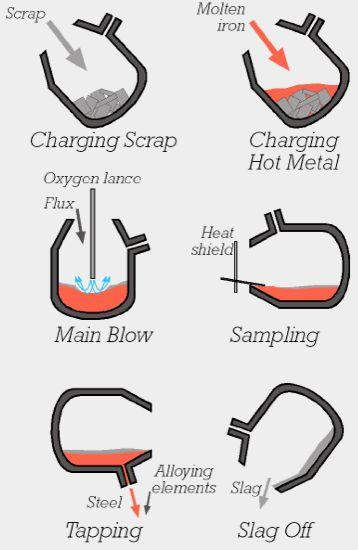
\includegraphics[width=.4\textwidth,angle=0]{convertor-phases.jpg}
	\caption{Znázornenie elementárnych procesov v LD konvertore.}
	\label{o:30}
\end{figure}

V závislosti od miestnych prevádzkových podmienok, dostupnosti šrotu, vysokopecného železa a rozsahu predúpravy, je kovová vsádzka do konvertora (LD/BOF, Q-BOP) tvorená 75 až 95 \% surovým železom a zvyšok je oceľový šrot. Používané druhy šrotu sú zvyčajne tie, ktoré sa vyrábajú v oceliarni: šrot z plechu, poškodené formy, plechovky a podobne \cite{Turkdogan1996}.

Kyslík je fúkaný vysokou rýchlosťou (až do dvojnásobnej rýchlosti zvuku) na povrch kovového kúpeľa v konvertore a v oblasti povrchu sa vytvára tzv. horúce miesto, kde prúd kyslíka naráža na povrch. Oxidačné produkty sa rozpustia v troske s výnimkou oxidu uhoľnatého, ktorý prechádza vrstvou trosky a tvorí hlavnú zložku konvertovaného plynu. Intenzita oxidácie jednotlivých prvkov závisí od ich chemickej afinity ku kyslíku. Oxidácia uhlíka je jedným z najdôležitejších procesov.

\begin{figure}[h!]
	\centering
	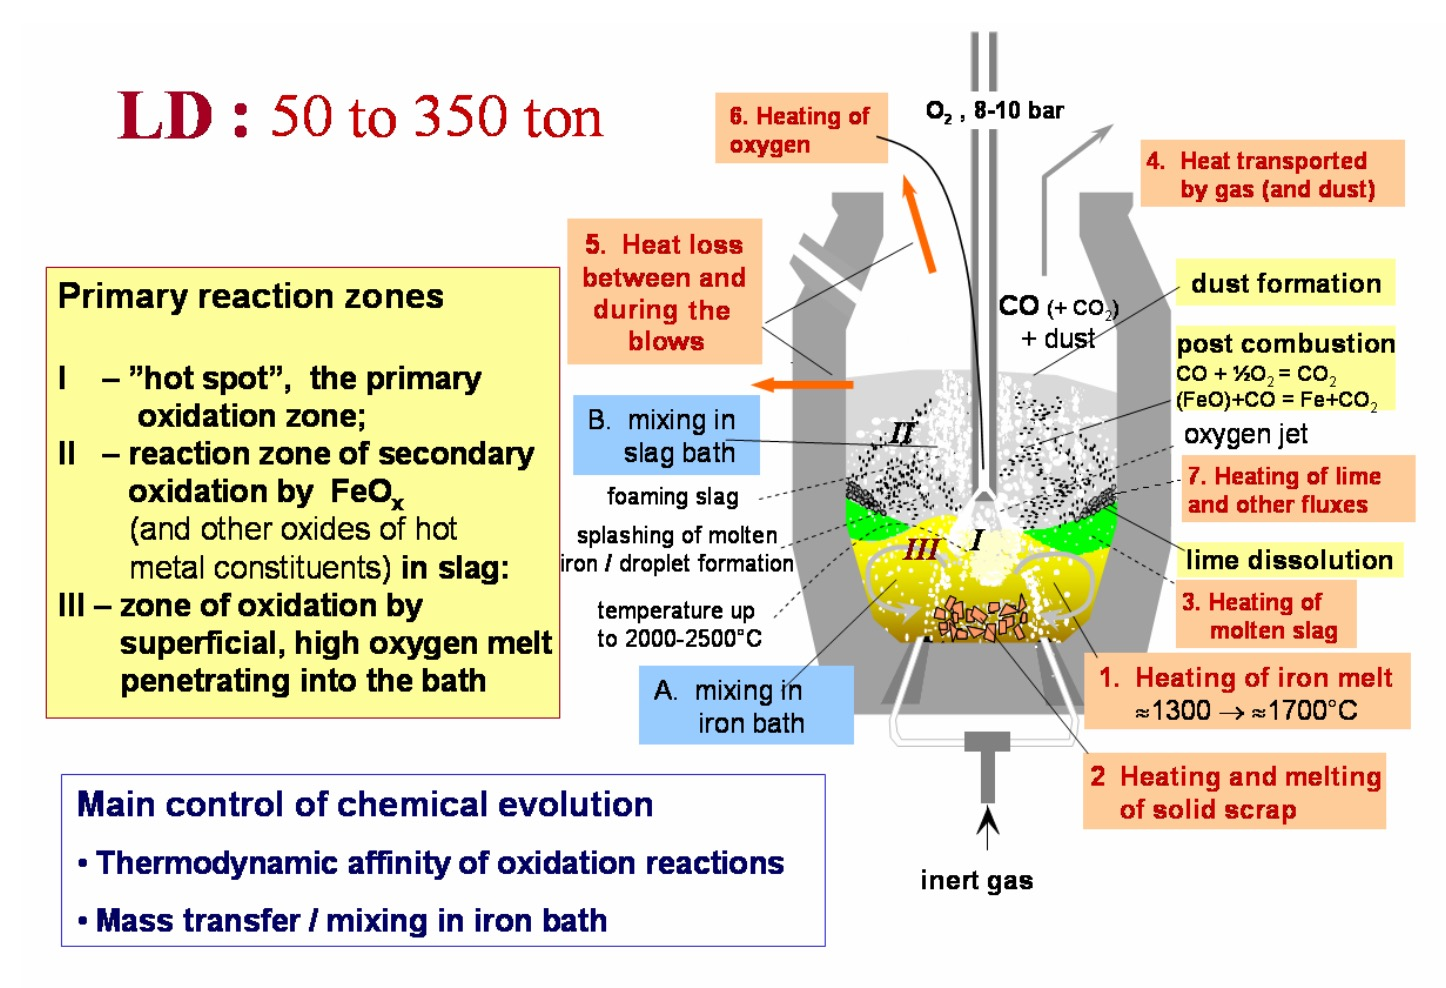
\includegraphics[width=1\textwidth,angle=0]{figures/ld-convertor-processes-graphical.jpg}
	\caption{Grafické znázornenie chemických a termodynamických procesov v LD konvertore \citep{Jalkanen2006}.}
\end{figure}

\section{Riadenie procesov v kyslíkovom konvertore}

Keďže cieľom výroby ocele v kyslíkových konvertoroch je spálenie (tzv. oxidácia) nežiadúcich nečistôt obsiahnutých v kovovej vsádzke, účelom tohto oxidačného procesu teda je:

\begin{itemize}
	\item znížiť obsah uhlíka na predpísanú úroveň (z približne 4 \% na menej ako 1 \%, ale často nižšie),
	\item upraviť obsah potrebných cudzích prvkov,
	\item odstrániť nežiadúce nečistoty v maximálne možnej miere.
\end{itemize}

Následnou úlohou riadiaceho procesu je potom získanie predpísaných parametrov ocele, ktorá sa odpichuje z konvertora, vrátane hmotnosti, teploty a obsahu každého prvku. Na základe týchto parametrov sa rozhoduje o tom, či je roztavená oceľ prijateľná alebo nie.

Počítačom podporované výpočty vsádzky sa robia pre každú tavbu. Asi 80 percent modelu riadenia vsádzky je založený na rovnováhe tepla a materiálu, zvyšok je založený na empirických vzťahoch, ktoré sa medzi jednotlivými taviarňami líšia. Pretože každá oceliareň má svoju vlastnú formuláciu modelu riadenia vsádzky \cite{Turkdogan1996}.

Za účelom monitorovania a riadenia procesu je možné použiť rôzne meracie systémy na poskytnutie spätnej väzby operátorovi alebo priamo existujúcemu systému na automatizované riadenie. Tieto merania môžu byť priame alebo nepriame, ako aj~s~časovým oneskorením alebo bez neho \cite{Widlund1998}.

\begin{figure}[h!]
	\centering
	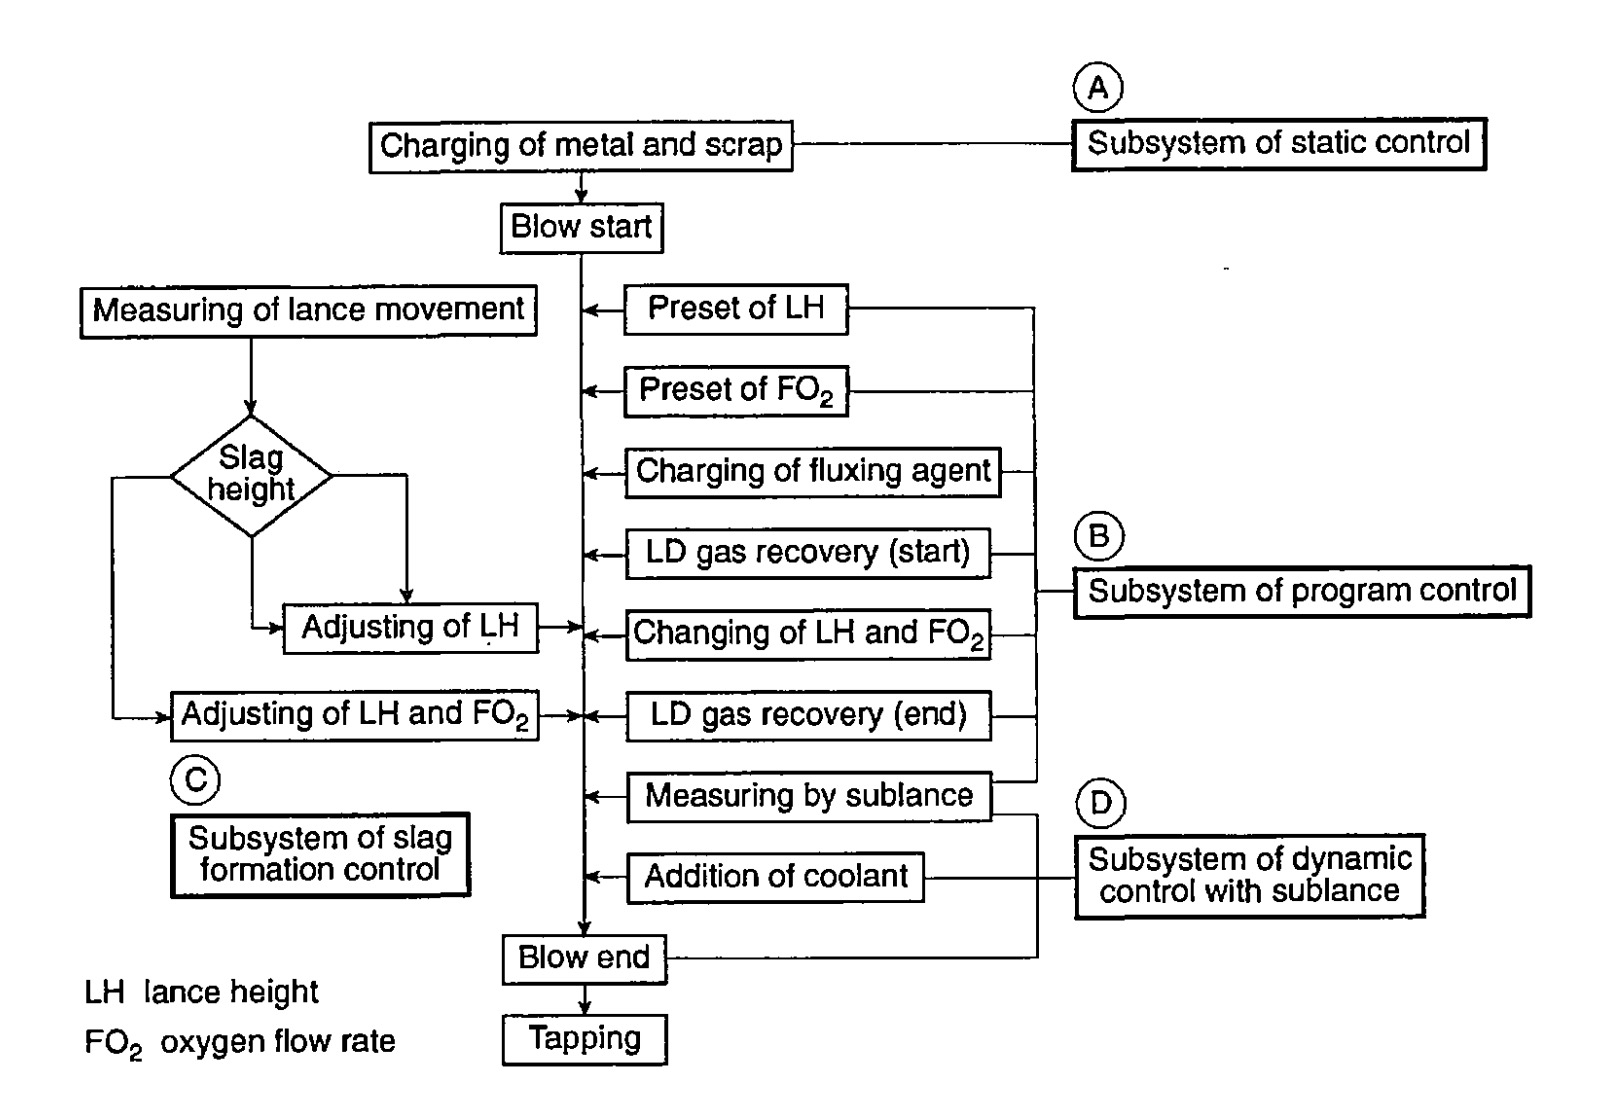
\includegraphics[width=.95\textwidth,angle=0]{figures/schematic-bof.jpg}
	\caption{Schéma funkcionality systému automatizovaného LD procesu \citep{Turkdogan1996}.}
\end{figure}

Existuje len niekoľko procesných premenných, ktoré môže nastavovať riadiaci systém alebo obsluha - výška trysky pre prívod fúkaného kyslíka, prietok kyslíka a~prietok čistiaceho plynu. Zmeny výšky prívodnej trysky sa merajú a nastavujú ľahšie, a preto je lepšie ich používať v riadiacom systéme s uzavretou slučkou. Zmena prietoku kyslíka počas LD procesu nesmie byť väčšia ako 5\%, pretože dýza je navrhnutá pre špecifický prietok \cite{Widlund1998}.

\subsection{Statický model riadenia}

Statický model riadenia je založený na celkovej materiálovej bilancii (Fe, troska, kyslík) a celkového tepla. Na základe prepočtov bilancií potom dostaneme informáciu o tom, koľko železnej rudy je potrebné pridať a aký objem kyslíka sa má dofúkať, spolu s konečnou hmotnosťou tekutej ocele a trosky pre dané hmotnosti, zloženie horúceho kovu a zloženie šrotu. Kvôli možnému vzniku chýb z dôvodu nerovnomernosti bilancie hmoty a tepla alebo neznámej časti týchto bilancií je tento model založený na spätnoväzobnom riadení.

\subsection{Dynamický model riadenia}

Dynamický model pre optimalizáciu riadenia procesov sa zameriava na dynamickú hmotnostnú bilanciu kyslíka, uhlíka a dusíka v spojení s množstvom prietoku a zloženia odpadového plynu. Je založený na pokročilých algoritmických rovniciach, ktoré popisujú komplexné termodynamické a metalurgické reakcie. 

Modely dynamického riadenia sú najčastejšie operujú na informáciách o odpadových plynoch a majú schopnosť predvídať stav procesu (zloženie ocele a trosky, ich hmotnosť, teplota) v akomkoľvek okamihu počas procesu. Na základe hmotnosti horúceho kovu a teploty sa vypočíta predikcia druhu a hmotnosti materiálu, ktorý je potrebné pridať na dosiahnutie požadovaného obsahu síry v horúcom kove. Pre optimalizovanie procesov fúkania kyslíka a miešania je využívaná komplexná simulácia kompletného LD procesu, ktorá je spúšťaná pred reálnou tavbou. Týmto spôsobom je možné zvoliť optimálnu stratégiu pre tieto procesy a zároveň optimálny čas a dávkovanie prísad. V ojedinelých prípadoch môže z prepočtov dynamického modelu vyplynúť potreba opakovať proces fúkania kyslíka prípadne ho len predĺžiť.

Ako príklad je možné uviesť jeden zo skupiny dynamických procesných modelov vyvinutý firmou Siemens VAI označovaný ako SteelExpert. Tento systém optimalizácie procesov je využívaný v LD konvertoroch v niekoľkých výrobných podnikoch v Číne, Južnej Afrike a na Slovensku (U.S. Steel Košice) \citep{siemensVAI}. Mimo vyššie spomínaných modelov, SteelExpert obsahuje modely ako FCC (first charge calculation), SCC (second charge calculation), Inblow, Supervision a LOMAS. FCC model určuje požadované množstvá rôznych druhov šrotu, ako aj množstvo horúceho kovu, ktoré má obsahovať vsádzka. SCC na základe skutočných údajov o horúcom kove a šrote vsádzanom do konvertora automaticky vypočíta požadovaný objem kyslíka a dávkovanie prísad pre požadovanú kvalitu ocele. Inblow využíva informácie z meraní vykonaných odbernou sondou priamo z tavby na vylepšenie modelu SCC prepočtom zvyšných vyhrievacích látok, chladiacich látok a zvyšného objemu kyslíka. Model Supervision cyklicky prepočítava reálny stav oceľového kúpeľa a trosky od skončenia vsádzky až po začiatok odpichu. Pre meranie odpadového plynu je využívaný systém LOMAS, ktorý vykonáva nepretržitú analýzu plynov počas spaľovacieho procesu pri vysokých teplotách a prašnosti. Analýza z inštalovaného hmotnostného spektrometra sa prenáša v dvoj-sekundových intervaloch a priamo sa využíva pri dynamickom riadení procesu. \newline

\begin{figure}[h!]
	\centering
	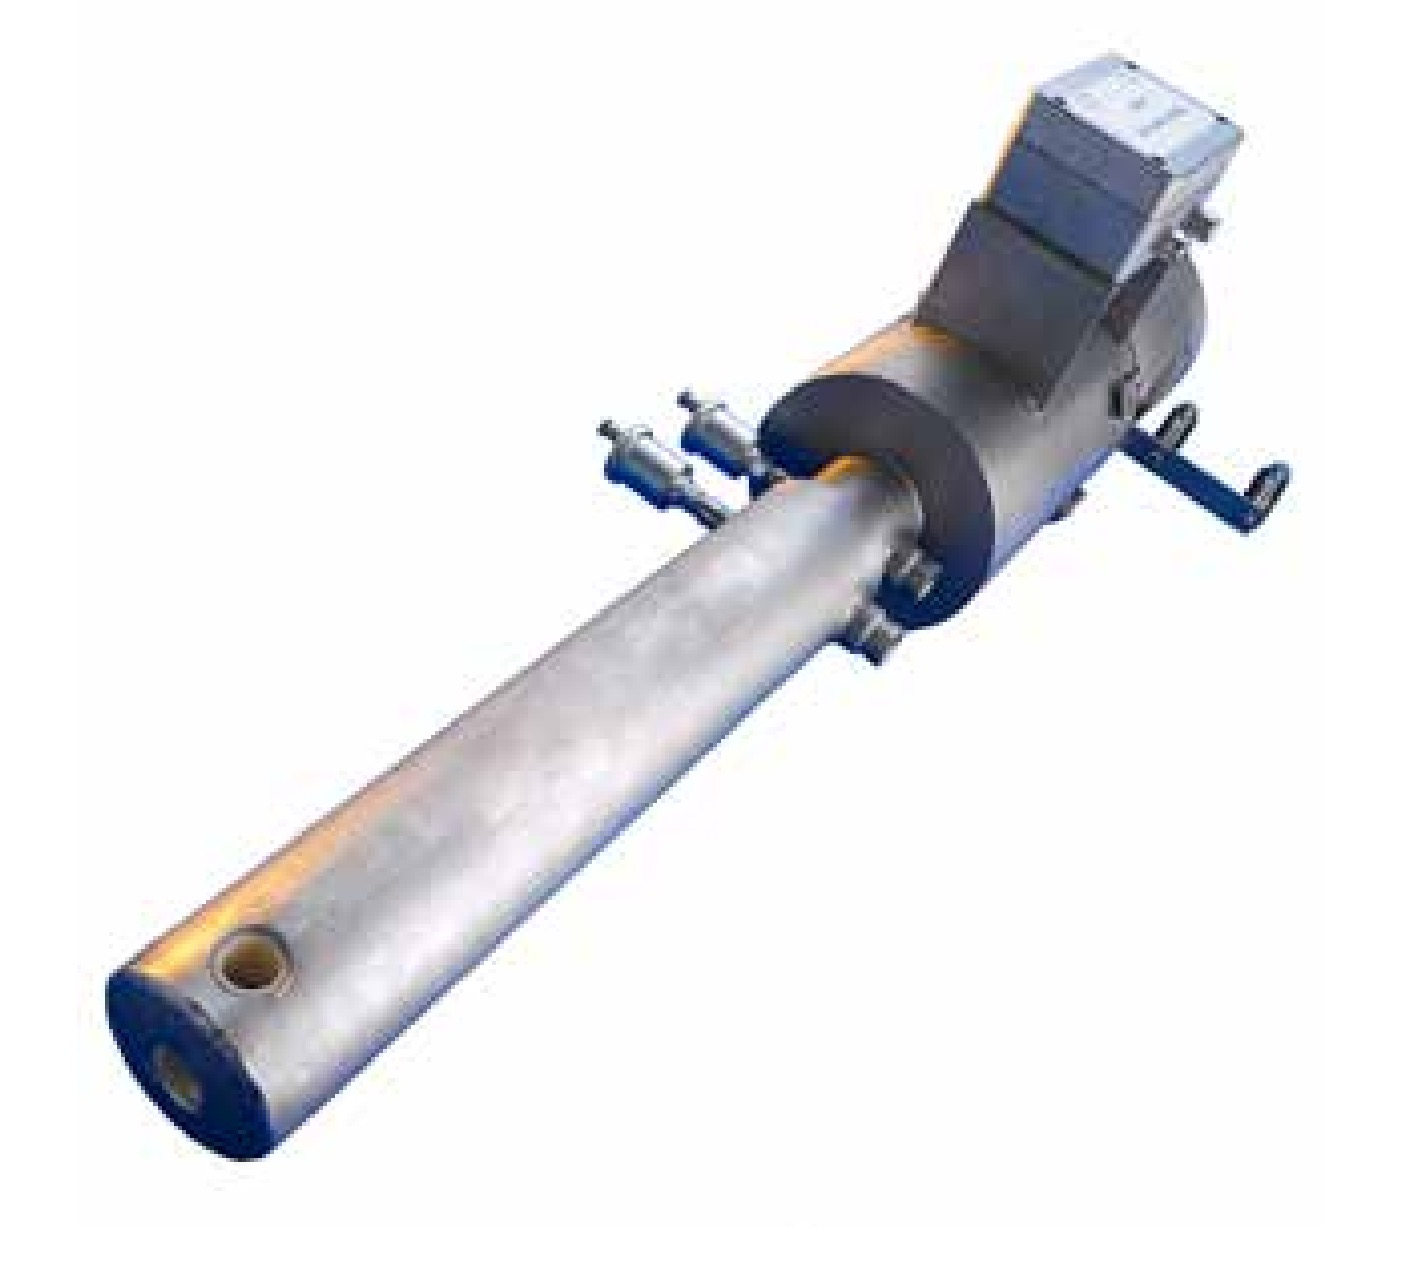
\includegraphics[width=.4\textwidth,angle=0]{figures/lomas-probe.jpg}
	\caption{Sonda LOMAS.}
\end{figure}

Výhody vyplývajúce z optimalizácie riadenia využitím dynamických modelov sú poznateľné zo štatistík vyhodnocovaných firmou Siemens VAI - uvádzajú 40\% redukciu odchýlky teploty, 45\% redukciu odchýlky obsahu uhlíka, zníženie potreby opätovného fúkania kyslíka o 60\% a zvýšenie produkcie ocele o 10\%.

\section{Automatizované riadenie procesov}

Plne optimalizovaná automatizácia riadiacich systémov je základom pre spoľahlivé výrobné procesy, maximálny výkon zariadenia a kvalitné výrobky, ktoré vyhovujú všetkým požiadavkám trhu. V súčasnosti si môžeme všimnúť posun priemyslu do novej paradigmy označovanej ako Priemysel 4.0, dôsledkom ktorej rastie počet podnikov, ktoré implementáciou inteligentných technológií zefektívňujú svoje procesy a znižujú náklady. Postupne sa na túto dráhu tzv. inteligentných výrobných podnikov dostávajú aj taviarne implementáciou inteligentnej diagnostiky stavu zariadení, monitorovanie výkonu a parametrov statického alebo dynamického modelu, ktoré sú vďaka väčšiemu množstvu senzorov lepšie zaznamenávané. Z dôvodu exponenciálneho nárastu objemu získavaných dát je kľúčové využitie umelej inteligencie, vďaka ktorej je možné z tohto množstva dát "vydolovať" cenné informácie s cieľom ešte viac zefektívniť riadenie procesov.

Systém automatizovaného riadenia LD procesu tvorí viacero podsystémov, akými sú naklápací pohon konvertora, merací systém s odbernou sondou, riadenie miešania horúceho kúpeľa, riadenie kyslíkovej dýzy, pneumatické zarážka trosky, váženie a kontrola prísad a zliatin, chladenie a čistenie odpadového plynu, zhodnotenie a analýza plynu, blokovací a poplachový systém. 

Jednotlivé podsystémy LD procesu sú riadené centrálnym PLC automatom s hlavným grafickým rozhraním (human-machine interface - HMI), ktoré monitoruje operatívny pracovník ale taktiež môžu byť menšie PLC integrované priamo do riadiaceho procesu daného podsystému.

\subsection{Naklápanie kovertora}

Úlohou naklápacích pohonov je rotácia nádoby konvertora do plniacej, vyprázdňovacej alebo vzorkovacej polohy. Pri naplnení LD konvertorov do maximálneho možného objemu tekutej ocele (s hmotnosťou 350-400 ton) váži konvertor celkovo cez 1000 ton. Na riadiaci systém takéhoto mechanizmu sú kladené vysoké nároky na spoľahlivosť a presnosť. Mechanizmus pohonu je vybavený v závislosti od veľkosti konvertora až štyrmi motormi (medzi ktoré sa rozdeľuje záťaž) s osobitnými frekvenčnými meničmi a riadením v uzavretej slučke. Riadiaci systém tak zabezpečuje funkčnosť pohonu aj v núdzových situáciách \citep{smsgroup}. 

\begin{figure}[h!]
	\centering
	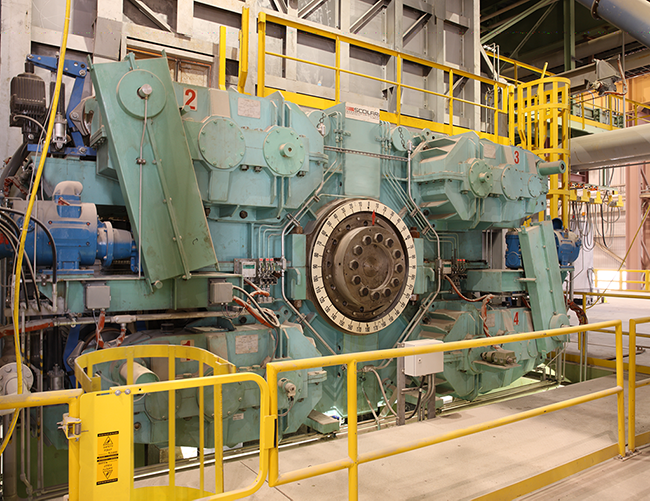
\includegraphics[width=.7\textwidth,angle=0]{figures/convertor-tilting-drive.png}
	\caption{Mechanika naklápacieho pohonu.}
\end{figure}

\subsection{Odoberanie vzoriek taveniny a meranie teploty}

Odberná sonda je dôležitým nástrojom pri výrobe ocele LD procesom. Poskytuje operátorovi cenné informácie o procese tavby akými sú teplota taveniny a jej zloženie. Zavádza sa automatizovane do vnútra konvertora cez bočný otvor kým je teleso konvertora v zvislej polohe, a to 2-krát počas tavby bez nutnosti jej prerušenia. Prvé zavedenie sondy zväčša býva po vyfúkaní 90\% objemu kyslíka vyčleneného pre danú tavbu, kedy sa meria teplota, objem uhlíka, zloženie trosky, výška oceľového kúpeľa a úrovne trosky. Druhé zavedenie sa uskutočňuje po procese fúkania.

\begin{figure}[!ht]
	\centering
	\subfloat[Odberná sonda od Berry Metal Company \citep{berrymetal}.]{{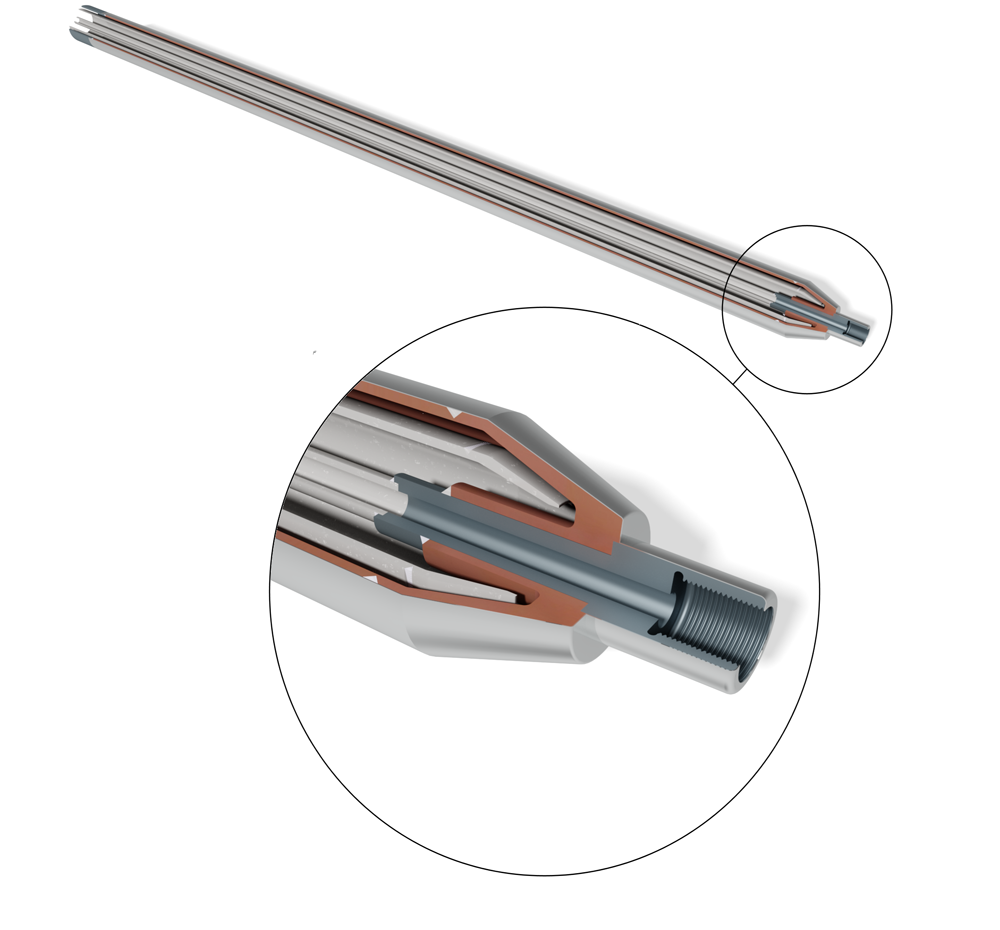
\includegraphics[width=6.5cm]{figures/sub-lance-berry.png} }}%
	\qquad
	\subfloat[Odber vzorky taveniny odbernou sondou v praxi.]{{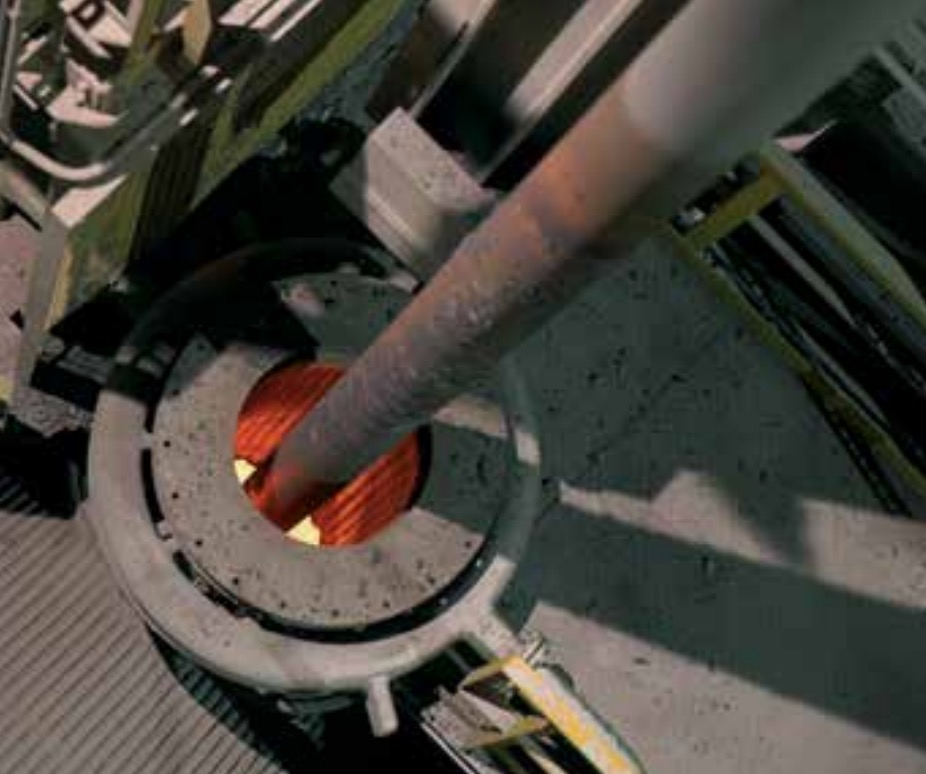
\includegraphics[width=7.35cm]{figures/sublance.jpg} }}
	\caption{Odberná sonda.}
\end{figure}

Moderné konvertory prevádzkujú merania odbernými sondami v spojení s kombinovaným statickým a dynamickým modelom riadenia procesu (SDM). Informácie získané z odbernej sondy sú ďalej spracované riadiacim systémom, ktorého optimalizačný model sa v konečnom dôsledku snaží o zvýšenie produkcie a dosiahnutie požadovaných vlastností ocele.

\begin{figure}[h!]
	\centering
	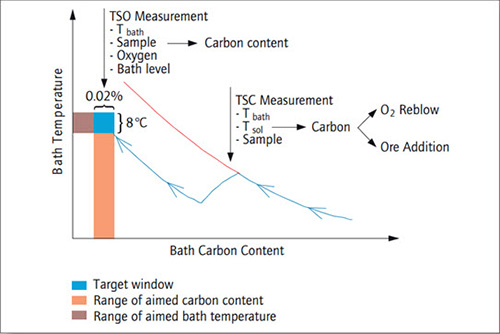
\includegraphics[width=.8\textwidth,angle=0]{figures/sublance-model.jpg}
	\caption{Statický a dynamický model riadenia procesu (SDM) merania odbernou sondou \citep{totalmateria}.}
\end{figure}

\subsection{Pneumatická zarážka trosky}

Aby sa zabránilo prenikaniu trosky z konvertora do panvy na konci odpichu, do otvoru je zvonku vrazená liatinová dýza, cez ktorú sa fúka zadržiavací plyn. Utesnenie sa vykonáva pneumaticky, a preto nie je ovplyvnené nepravidelným opotrebovaním otvorov a konzistenciou trosky. Spoľahlivé utesnenie je možné pomocou ľubovoľnej trosky. Detekcia trosky a proces uvedenia zarážky do činnosti sú spúšťané automaticky pomocou systému ``IRIS" (infračervená indikácia trosky). Tento systém vyhodnocuje rozdiely infračerveného žiarenia ocele a trosky, ktoré sa zaznamenávajú pomocou infračervenej kamery.

\newpage

\begin{figure}[!ht]
	\centering
	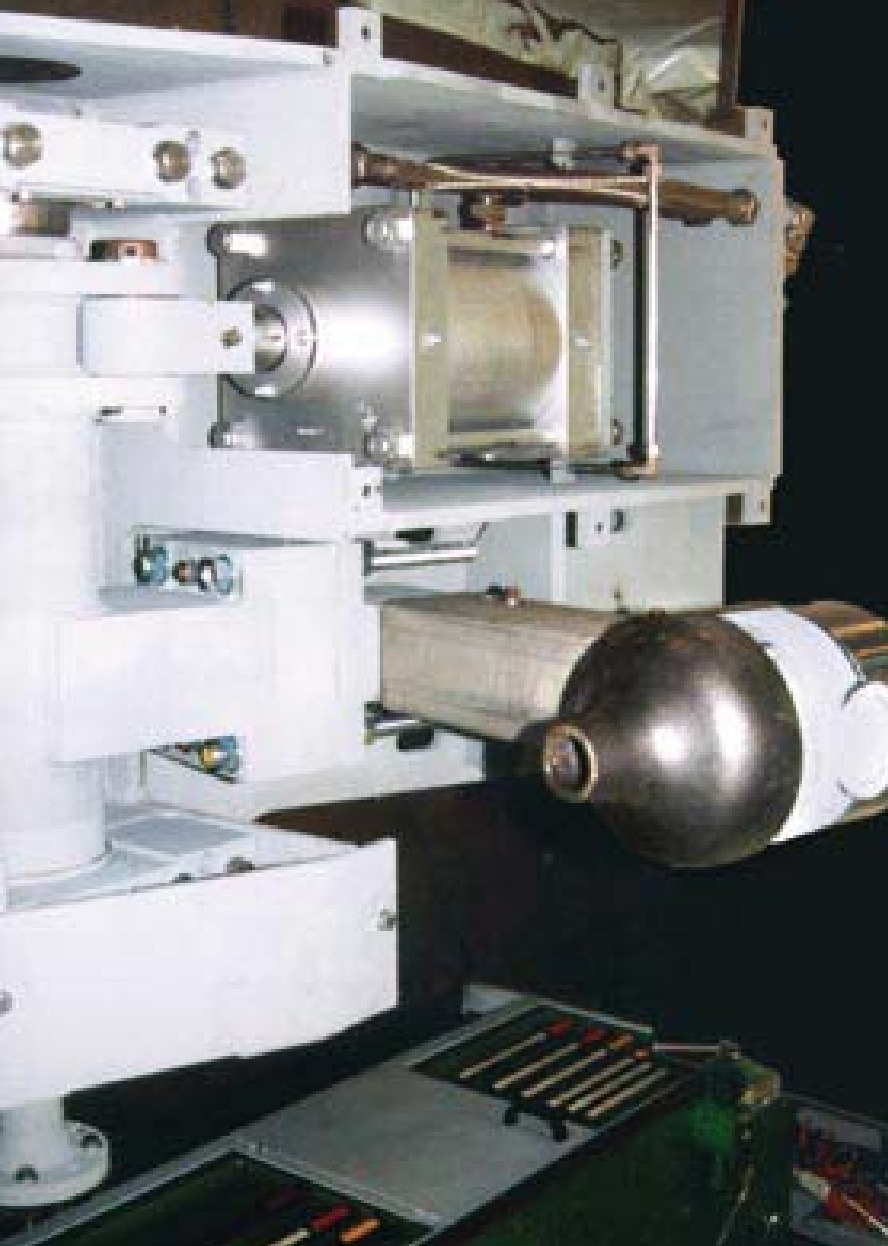
\includegraphics[width=.5\textwidth,angle=0]{figures/slag-stopper.jpg}
	\caption{Statický a dynamický model riadenia procesu (SDM) merania odbernou sondou \citep{totalmateria}.}
\end{figure}

\subsection{Spodné miešanie horúceho kúpeľa}

Miešanie zdola pomocou inertného plynu ponúka výhody v metalurgických a prevádzkových aspektoch. Predovšetkým sa výrazne zlepšuje kinetika procesu a je možné dosiahnuť oduhličovaciu reakciu aj pri nízkom obsahu uhlíka. Riadenie toku inertného plynu je riešené individuálne s rovnomerným rozdelením toku medzi viacero trysiek, čo ponúka optimálnu bezpečnosť pri práci a lepšiu obsluhu. Efektivita procesu miešania výrazne závisí od konfigurácia trysiek na spodnej časti konvertora \citep{Choudhary2006}.

\begin{figure}[h!]
	\centering
	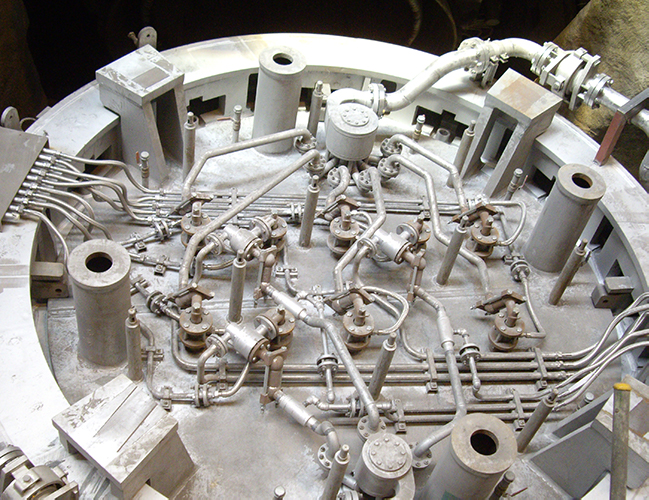
\includegraphics[width=.7\textwidth,angle=0]{figures/bottom-stirring-tuyeres.jpg}
	\caption{Spodná časť konvertora.}
\end{figure}

\newpage

Rovnomerné rozdelenie prúdu plynu medzi každým miešacím prvkom zaisťuje rovnomerný chladiaci účinok, čím sa zabraňuje opotrebeniu jednotlivých miešacích prvkov. Prietok a typ miešaného plynu (dusík alebo argón) závisí od výrobnej fázy, požadovanej kvality ocele a jej zloženia, v závislosti ktorého sa môže vyžadovať prechod z dusíka na argón alebo opačne. Jednou z častí systému miešania je ventilová stanica, ktorej potrubia vedú do konvertora a ktorá umožňuje individuálne riadenie prietoku na jednotlivé preplachovacie zátky.

\begin{figure}[h!]
	\centering
	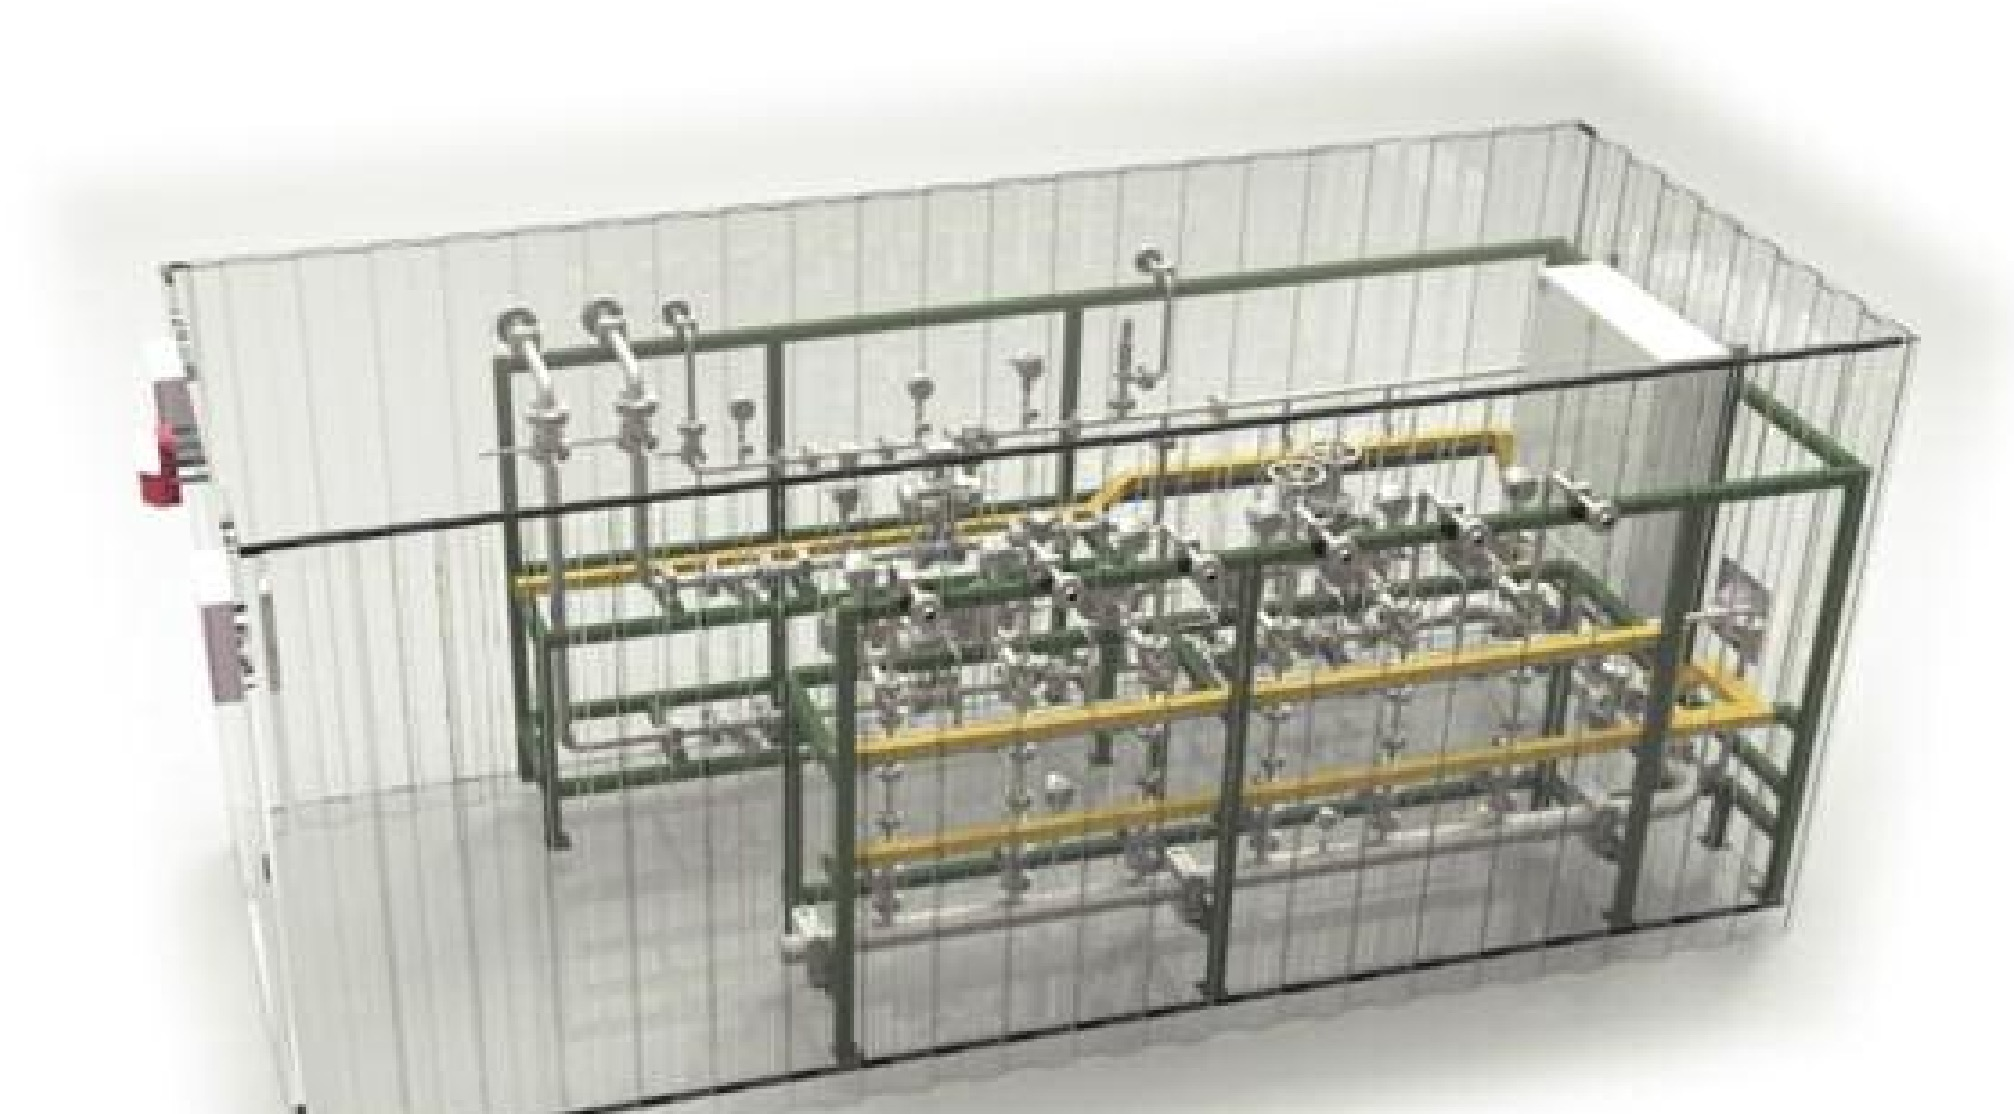
\includegraphics[width=.6\textwidth,angle=0]{figures/valve-station.jpg}
	\caption{Ventilová stanica.}
\end{figure}

%
%%
\Urlmuskip=0mu plus 1mu\relax
\bibliographystyle{spbasic}
\bibliography{refs/control,refs/mathematics,refs/modeling,refs/cfd,refs/lbm,refs/gpu,refs/interaction,refs/interfaces,refs/hci,refs/design,refs/ml,refs/visualization,refs/programming,refs/simulation,refs/ar,refs/vr,refs/online}

%

\end{document}
%%